\chapter{Batch RL}
\label{chapter:batchrl}

We decide to test the capabilities of our algorithm in a \textit{fully} off-policy setting, 
also called \textit{batch RL setting} or \textit{offline RL}. In this setting, the agent 
can only learn from a fixed dataset without further interaction with the environment.

Most of RL algorithms provide a fundamentally \textit{online} learning paradigm which involves
iteratively collecting experience by interacting with the environment, and then
using that experience to improve the policy. 
In many  real-world scenarios, continuous interacting with the environment is impractical, either because 
data collection is expensive, as in robotics or healthcare, or dangerous, for example a physical robot may
get its hardware damaged or damage surrounding objects.
Additionally, even in some cases were online interaction is feasible, we might prefer to still use previously
collected datasets - for example, if the domain is complex (such as a robot learning to cook several meals at home)
and effective generalization (e.g cooking in different kitchens or using different ingredients for the meal)
requires large datasets \cite{levine2020}.


The ``off-policy" algorithm we presented in previous sections, and similarly to most of the ``off-policy"
algorithms in literature, falls in the category of 
off-policy \textit{``growing batch learning"}. In this case, agent's experience is appended to a data buffer 
$\mathcal{D}$ and each new policy $\pi_k$ collects additional data, such that $\mathcal{D}$
is composed of samples from $\pi_0,\pi_1...,\pi_k$ and all of this data is used to train an update new
policy $\pi_{k+1}$. 
%As a result, the training data tends to be heavily correlated to the current policy.
Hence, despite being off-policy these methods require active online data collection.

In contrast, in offline RL the agent no longer has ability to interact with the environment and collect
additional transitions. Instead, it
can only employ a static dataset $\mathcal{D}$ collected by an external agent using policy $\pi_\beta$
and must learn the best policy it can only using this dataset.

In numerous real-world applications, such as games or robotics, there is already plentiful amounts 
of previously collected interaction data which are a rich source of prior information.
RL algorithms that can train agents using these prior datasets without further data collection
will not only scale to real-world problems, but will also lead to solutions that generalize substantially better.
Off-line RL holds tremendous promise for making it possible to turn large datasets into powerful 
decision-making engines, effectively allowing anyone with a large enough dataset to turn this dataset
into a policy than can optimize a desired utility criterion. \citep{levine2020}.


\section{Issues with Batch RL} \todo{change title?}

Most of recent off-policy algorithms such as Soft Actor-Critic \citep{Haarnoja2018}, 
DDPG \citep{Lillicrap2016} and Rainbow \citep{Hessel2018}  could be in principle used 
as an offline RL algorithm, i.e. learn from data collected from an unknown behavioral policy
$\pi_\beta$ with state visitation frequency $d^{\pi_\beta}(s)$. 
However, in practice, they still require substantial amounts
of “on-policy” data from the current behavioral policy in order to learn effectively, 
and generally they fail to learn in the off-line setting.

This is due to a fundamental problem of off-policy RL, called \textit{distributional shift}, which in 
its turn induces what's called extrapolation error \citep{Fujimoto2019} or bootstrapping error \citet{Kumar2019}.\\
Distributional shift affects offline RL via dynamic programming algorithms (as ours, i.e. methods aiming
to learn a state or state-action value function), both at test time and training time.
State distribution shift affects test-time performance, but no training, since neither the policy nor
the Q-function is ever evaluated at any state that was not sampled from $d^{\pi_\beta}$.\\
However, training process is indeed affected by \textit{action distribution shift}.
This is because when doing the Bellman backup to update the Q-function estimate,
the \textit{target} values require evaluating the estimated $Q^\pi(x_{k+1},a_{k+1})$ where
a is chosen according to current policy $\pi$.
Since targets are computed via bootstrapping, accuracy of Q-function regression depends
on the estimate of the Q-value at these actions. When $\pi$ differs substantially from $\pi_\beta$, 
these actions are generally unlikely or not contained in the dataset, i.e.
out of the distribution of actions that Q-function was ever trained on. This can result
in highly erroneous targets Q-values, and in its turn, in updated new Q estimates 
with pathological values that incur large absolute error from the optimal desired Q-value.\\
This issue is further exacerbated when $\pi$ is explicitly optimized to maximize $Q^\pi(s,\pi(a))$.
Then, the policy will learn to produce out-of-distribution (OOD) actions
for which the learnt Q-function erroneously overestimates.
This source of distribution shift is in fact one of the largest obstacles for practical application
of dynamic programming methods to offline RL.

It is important to notice that for on-policy settings, extrapolation error is generally something positive, since it
leads to a beneficial exploration. In this case, if the value function is overestimating the value at
a (state-action) pair, the current policy will lead the agent to that pair and will observe that in fact
it is not as good and hence, the value estimate will be corrected afterwards.
However, in the offline setting, the correction step on such over-optimistic Q-values cannot be done by the 
policy, due to the inability of collecting new data, and these errors accumulate over each iteration of training,
resulting in arbitrarily poor final results or even divergence.


To address this OOD actions problems and effectively implement offline RL via dynamic programming,
\citet{Fujimoto2018} opted for constraining the trained policy distribution to lie close to
the dataset policy distribution, to avoid erroneous Q-values due to extrapolation error.
\citet{Kumar2019} suggested a less restrictive solution to constrain the learnt policy to lie
\textit{within the support} of the dataset policy distribution.
\todo{maybe cite more?}

For our algorithm, we will inspire ourselves in the approach presented in 
\citet{Fujimoto2019}, which we introduce below with its further modifications.


\section{Our approach} \todo{more explicit title?}
In \citet{Fujimoto2019}, they present a Batch-Constrained Deep Q-learning (BCQ)
algorithm in which they
train a generative model $G_w$ to generate actions with high similarity to the dataset.
For the generative model they use a conditional variational auto-encoder (VAE) \cite{Kingma2014} which
generates action samples as a reasonable approximation to
$\underset{a}{\text{argmax}}  P _\mathcal{B}^G(a|x)$, where $P_\mathcal{B}^G(a|x)$ is 
the state-conditioned marginal likelihood given the (state-action) pairs in the 
batch $\mathcal{B}$.
\citet{Fujimoto2019} presents a Q-learning approach, for which
they sample multiple candidate actions from the VAE, they perturbed them via a perturbation model
and select the highest valued-action 
according to a learnt Q-network.

For our approach, we only use from \citet{Fujimoto2018} the VAE network to sample actions similar to
the dataset, which are then perturbed to maximize the CVaR of the return distribution.
The rest of the algorithm keeps intact as the one we presented, and as later summarized.

We proceed to explain how we update our Distributional off-policy deterministic actor-critic algorithm previously
presented to be able to learn effectively in the Batch RL setting.

We generate actions using a  variational autoencoder $G_w$,
which is trained to generate actions $\hat{a}$ with high  similarity  to  the  dataset.  
Afterwards, we perturb $\hat{a}$  to generate actions $a$ that maximize the CVaR of the return
distribution. This perturbation is done by a perturbation model  or actor network, $\xi$, which is trained in
the same way as the previously presented actor network,
i.e. to maximize the CVaR of the estimated return distribution via deterministic gradient ascent.

\begin{align}
    \hat{a_i} \sim G_w(x)\\
    a_i =  \hat{a_i} + \xi(x,\hat{a_i};\phi,\theta^\xi)
\end{align}

where  $\xi(s,a;\phi)$ is a perturbation model that outputs an adjustment to action $\hat{a}$
in the range $[-\phi,\phi]$. $\phi$ is a fixed parameter which determines how much imitation learning
is used for the final actions. Low values of $\phi$ will reduce the perturbation and hence the 
learnt policy will behave more closely to the behavior policy used to obtain the dataset.



\subsection{Details of Conditional VAE}
For the generative model $G_w$, we use a conditional variational autoencoder $G_w$.
Given state-action pairs $x^B,a^B$ from the dataset, the conditional variational autoencoder
aims to maximize the state-conditioned marginal log-likelihood  
$\log P_\mathcal{B}(A|X) = \sum_{i=1}^{N}\log  P_\mathcal{B}(a_i|x_i)$.
Hence, using the trained generative model we can sample actions
as a reasonable approximation to $ \arg \underset{a}\max P_\mathcal{B}^G(a|x)$, ie very similar to 
the actions from the dataset.

It is assumed that the data is generated by some random process, involving an unobserved continuous
random variable \textbf{z}.
The process consists of two steps: (1) a value \textbf{$z_i$} is generated from some prior distribution p(z) and (2)
an action $a_i$ is generated from some conditional distribution $p(a|z,x)$. 
The state $x$ is also included given the fact we are modelling the state-conditioned
likelihood $P_\mathcal{B}^G(a|x).$
Given that the true probabilities are unknown, a recognition model $q(z|a,x; \phi )$ is introduced
as an approximation to the intractable true posterior $p(z|a,x; \theta)$.\\
The recognition model $q(z|a,x; \phi)$ is called an \textit{encoder},  since given a datapoint $(x,a)$ it produces
a \textit{random latent vector} z.
$p(a|z,x; \theta)$ is called a \textit{decoder},
since given the random latent vector z (and state x) it reconstructs the original sample a.\\
Since computing the desired marginal $P_\mathcal{B}(A|X; \theta)$ is intractable, VAE algorithm optimizes a lower bound instead:
\begin{align}
    &\log p(A|X; \theta) \geq \mathcal{L}(\theta, \phi; A|X) \\
    &\mathcal{L}(\theta, \phi; A|X)=\mathbb E_{q(z|A,X;\phi)} [\log p(A|z,X; \theta)] - D_{KL}(q(z|A,X;\phi)\; ||\;p(z; \theta)) \label{eq:vae_loss}
\end{align}

\section{Batch RL Distributional DeterministicOff-policy Actor-critic algoritm for CVaR otpimization}

For our implementation, the prior $p(z; \theta)$ is chosen to be a multivariate normal
distribution $\mathcal{N}\big( 0,Id\big )$, hence it doesn't require parameters $\theta$.
\todo{caption add name of alg}
\begin{figure}[ht]
    \centering
    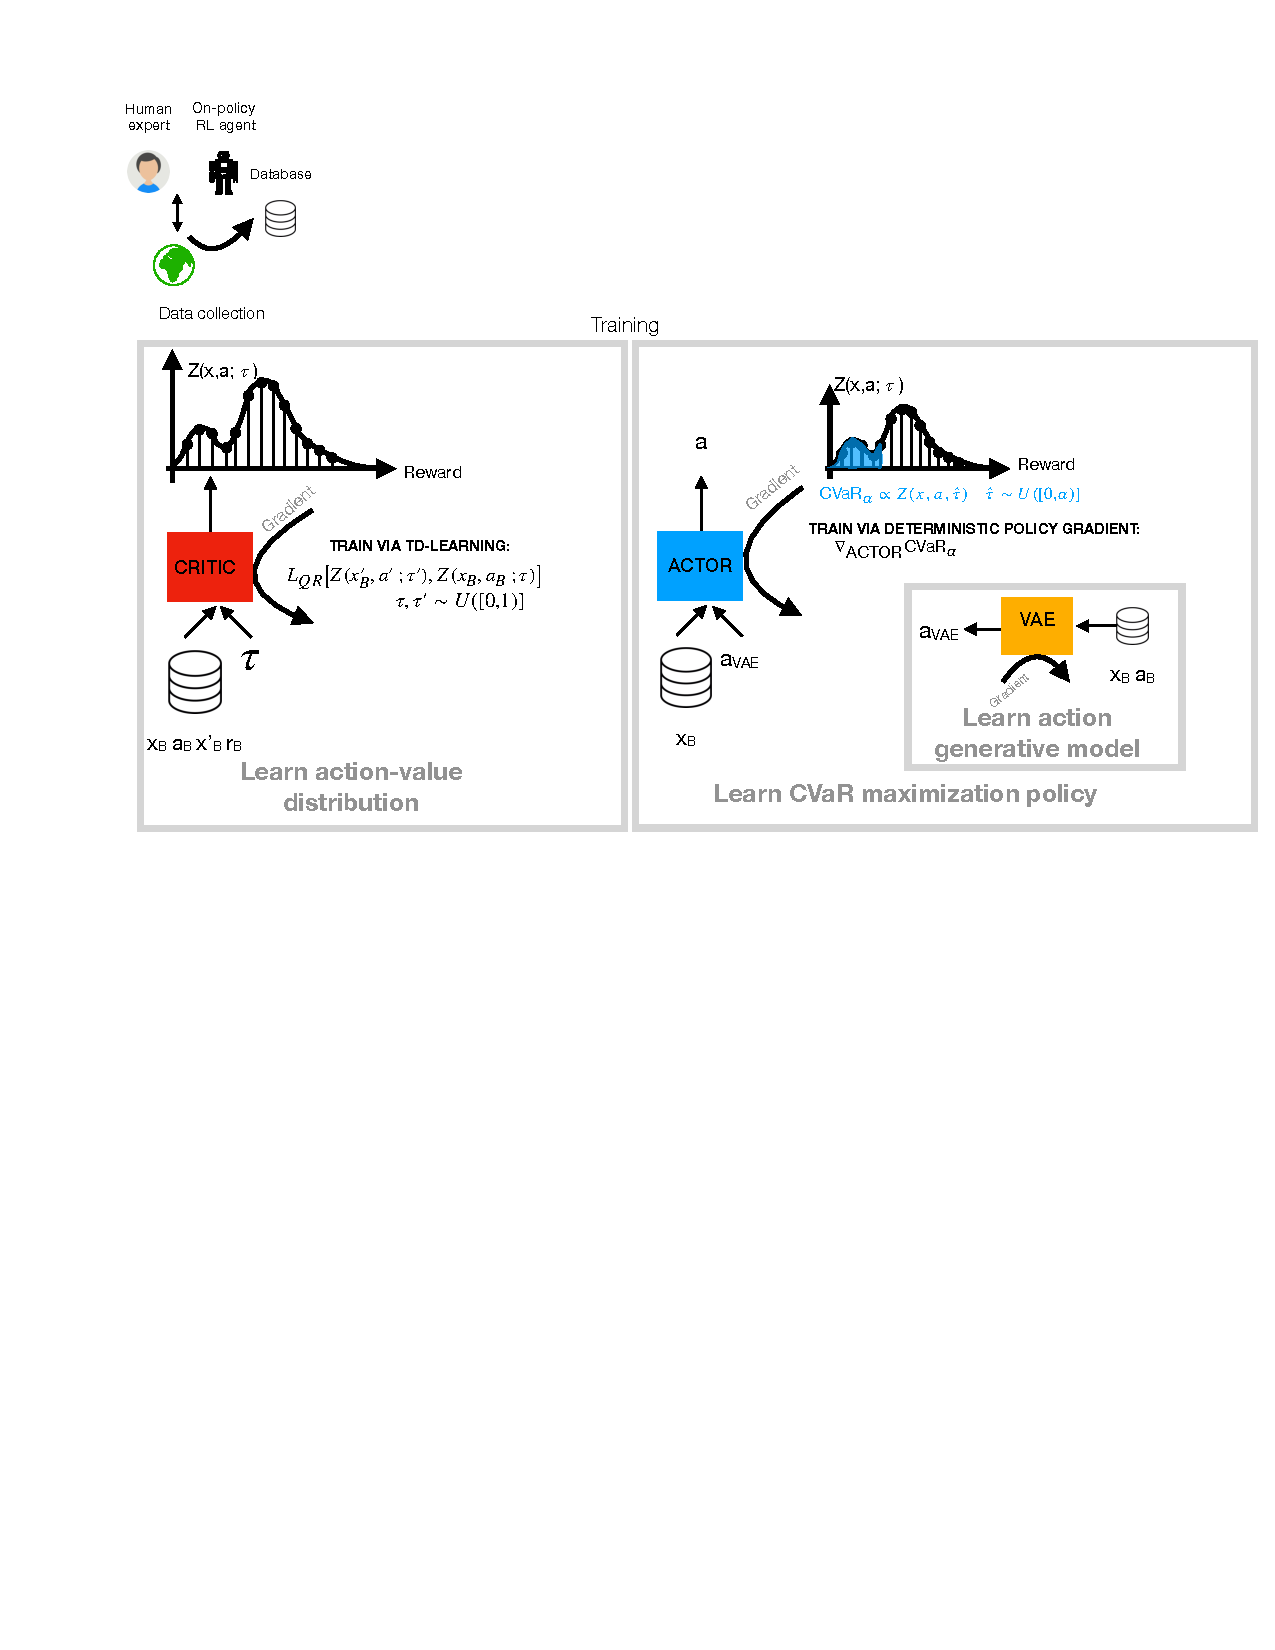
\includegraphics[width=0.8\textwidth]{images/diagram.pdf}
    \caption{Graphical representation of the algorithm.
    Algorithm is implemented fully off-policy using an external training dataset obtained
    for example, by a human expert or an on-policy RL algorithm.
    Algorithm consists in 3 main blocks: the \textit{VAE generative model}, the \textit{actor}
    and the \textit{critic}.
    The \textit{VAE generative model} learns to generate actions similar to actions present in the training dataset.
    The \textit{critic} learns 
    the action value distribution via quantile regression TD-learning.
    The \textit{actor} learns a policy to maximize the CVaR by perturbing the actions 
    generated by the generative model towards risk-sensitive actions and it is trained
    via deterministic gradient ascent of the CVaR computed by sampling from the 
    estimated parameterized action-value distribution.}
    \label{fig:diagram}

\end{figure}
For the probabilistic encoders and decoders we use neural networks.
For the encoder $q(z|a,x;\phi)$ we used a neural network with  Gaussian output, specifically a 
multivariate Gaussian with a diagonal covariance structure $\mathcal{N}(z | \mu(a,x;\phi), \sigma^2(a,x)Id ; \phi)$,
where $\mu$ and $\sigma$ are the outputs of the neural network, i.e. nonlinear 
functions of datapoint $(x_i,a_i)$ and $\phi$.
To sample from the posterior $z_i \sim q(z|a,x; \phi)$ we use the reparameterization trick:
\begin{equation}
    z_i = g(a_i,x_i, \epsilon; \phi)=\mu_i + \sigma_i \odot \epsilon \quad \epsilon \sim  \mathcal{N}(0,Id)
\end{equation}
where $\odot$ is the element-wise product.

For the decoder $p(a|z,x; \theta)$ we used another neural network with deterministic output, i.e. nonlinear function of 
datapoint $(x_i,z_i)$ and $\theta$.

When training the VAE, both recognition model parameters $\phi$ and the generative model parameters $\theta$ are
learnt jointly to maximize the variational lower bound $\mathcal{L}(\theta, \phi; X)$ in \ref{eq:vae_loss} 
via gradient ascent, i.e. maximize expected reconstruction loss and a KL-divergence term
according to the distribution of the latent vector z.

When both prior and posterior are Gaussian, KL-divergence can be computed analytically:
\begin{equation}
    D_{KL}(q(z|X;\phi)\; ||\;p(z; \theta)) = -\frac{1}{2}\sum_{j=1}^J (1+\log((\sigma_j)^2)-(\mu_j)^2-(\sigma_j)^2) \label{eq:kl_div}
\end{equation}

where J is the dimensionality of z, and $\mu_j,\sigma_j$ represent the j-th element of the vectors.\\
The expected reconstruction error 
$\mathbb E_{q(z|X;\phi)} [\log p(X|z; \theta)]$
requires estimation by sampling. We use the mean-squared error between the action $a_\mathcal{B}$
from the dataset and the reconstructed action.

Finally, when generating actions during evaluation or deployment, random values of z are sampled from a
multivariate normal and passed through the decoder to produce the actions.



The perturbation model is trained as in \ref{eq:alg2}:
\begin{align}
    \nabla_{\theta^\xi} J_\beta(\xi | \theta^\xi) &\approx \mathbb E_{x \sim \rho^\beta} 
\big [\nabla_{\theta^\xi} \xi(x,\hat{a}| \theta^\xi) \nabla_a  [\frac{1}{\alpha} \frac{1}{K}
\sum_{i=1}^K Z(x,a; \tau_i) | \theta^Z)]|_{a=\xi(x,\hat{a}| \theta^\xi)}  \big] \label{eq:algbatchrl_2}
\end{align}

Figure \ref{fig:diagram} shows a graphical representation of the algorithm with its 3 main parts:
the generative model learning to generate actions similar to the ones in the dataset,
the critic learning the value distribution and the actor learning the CVaR maximization policy
by perturbing the actions generated by the generative model towards risk-sensitive ones.


\section{Technical details}
Algorithm works very similarly to the off-policy RL previously presented, and hence shares almost all details
as the ones introduced in \ref{sec:technical_details}.
We focus here on the differences or new additions.
For batch RL, we do not need to account for exploration so there is no such behavior policy.
At every training-step a minibatch of observations  $(x_t^B,a_t^B,r_t^B,x_{t+1}^B)$ is sampled from
static dataset.

Given $x_{k}^B,a_{k}^B$ from the dataset and the generative model $G_w$ with its encoding $E_w$ and decoding $D_w$
we sample actions $hat{a}_k^{VAE}$ from the conditional VAE by:

\begin{align}
    \mu, \sigma, z = E_w(x_{k}^B,a_{k}^B) \quad \text{where} \; z=\mu + \sigma \mathcal{N}(0,Id)\\
    \hat{a}_k^{VAE} = D_w(x_{k}^B, z)
\end{align}
Then we train jointly $[E_w,D_w]$ via gradient descent:
\begin{align}
    \mathcal{L}^{VAE}(E_w,D_w)= \sum_k[\hat{a_k}^{VAE}-a_{k}^B]^2 + 0.5 D_{KL}
\end{align}
where $D_{KL}$ is computed as in \ref{eq:kl_div} using $\sigma,\mu$ from the outputs of the encoder.

Actor or \textit{perturbation model} training is done by gradient ascent as in \ref{eq:algbatchrl_2}
where 
\begin{equation}
    \hat{a} = D_w(x^B, z_{CLIP}) \quad z_{CLIP} = \text{clip}(z, -0.5,0.5) \;z \sim \mathcal{N}(0,Id)
\end{equation}

We train the critic in the same way as the original algorithm,
using a critic target network to estimate the target values 
which slowly tracks the learnt networks.
$a_{k+1}$ actions used to compute target Z values $Z(x_{k+1}^B,a_{k+1}; \tau_i)$,
are computed as the output of the perturbation model $\epsilon$, which also uses a target network.

During deployment, the stochasticity of the policy due to sampling the latent vector z from 
$z \sim \mathcal{N}(0,Id)$ can be removed by setting $\sigma=0$.



\begin{algorithm}[H]
    \DontPrintSemicolon
    \SetAlgoLined
    \textbf{Input:} Training dataset $\mathcal{B}$, quantile levels $N',N, K$, minibatch size $n$,
    $\alpha$ confidence, $\Phi$ perturbation level\;
    
    \textbf{Initialize:} Critic network $Z$, VAE network $G=\{E_G,D_G\}$ and actor network
    $\xi$ parameters and target networks $Z'\leftarrow Z$,
    $\xi' \leftarrow \xi$ parameters
    
    \While{training}{
      Sample minibatch of $n$ transitions ($x_\mathcal{B},a_\mathcal{B},x'_\mathcal{B},r_\mathcal{B}$)
      from the dataset $\mathcal{B}$\\
      \textcolor{mygray}{Train variational autoencoder:}\
        $\mu,\sigma = E_G(x_\mathcal{B},a_\mathcal{B})\quad \hat{a}^{VAE}=D_G(x_\mathcal{B},z) \quad z=\mathcal{N}(\mu,\sigma)$\
        $\theta^G \leftarrow \text{argmin}_{theta^G} \sum (a-\hat{a}^{VAE})^2 + \text{D}_{KL}(\mathcal{N}(\mu,\sigma)||\mathcal{N}(0,1))$\\
     
      \textcolor{mygray}{Train critic:}\;
        $\tau_i, \tau'_j \sim U([0,1]) \quad 1\leq i,j \leq N,N'$\\
        Compute next action a':\\
        $\hat{a}'^{VAE} \sim{G_w(x'_\mathcal{B})}$\\
        $a'=\hat{a}'^{VAE} + \xi'_\Phi(\hat{a}'^{VAE}, x'_\mathcal{B})$\\
        Compute distributional TD: $\delta_{ij}=r+ \gamma Z'(x'_\mathcal{B}, a';\tau'_j) - Z(x_\mathcal{B}, a_\mathcal{B};\tau_i) \; \forall i,j$\\
        $\theta^Z \leftarrow \text{argmin}_{\theta_Z} \sum_{i=1}^{N}\mathbb E_{\tau'}[\rho_{\tau_i}(\delta_{ij})]$\;
    
      \textcolor{mygray}{Train actor:}\;
        $\tau_k \sim U([0,\alpha]) \quad 1\leq k \leq K$\\
        $\hat{a}^{VAE} \sim{G_w(x_\mathcal{B})}$\\
        $a=\hat{a}^{VAE} + \xi_\Phi(\hat{a}^{VAE}, x_\mathcal{B})$\\
        Compute $\text{CVaR}_\alpha=\frac{1}{\alpha K}\sum_{k=1}^K Z(x_\mathcal{B},a;\tau_k)$\\
        $\theta^\xi \leftarrow \text{argmax}_{\theta_\xi} {CVaR}_\alpha$\;
      \textcolor{mygray}{Update target networks:}\;
        $\theta^{Z'}\leftarrow \tau\theta^Z + (1-\tau)\theta^{Z'} $;
        $\theta^{\xi'}\leftarrow \tau\theta^\xi + (1-\tau)\theta^{\xi'} $\\
    }
    \label{pseudocode:algo2}
    \caption{$\thenameoff$}
\end{algorithm}
    